% ch01_intro.tex : Introduction chapter
% Dr. Yael Mizrahi : LaTeX Technical Author
% ≥2500 words, ≥4 subsections, ≥2 equations, ≥3 citations

\selectlanguage{hebrew}

\section{מבוא : ניווט רחפנים בהשראת עטלפים באמצעות מיזוג חיישנים רב-מודאלי ביומימטי}
\label{sec:intro}

\subsection{רקע ומוטיבציה}
\label{sec:background}

ניווט רחפנים בסביבות נטולות \en{GPS} נותר אחד האתגרים המרכזיים ברובוטיקה אוטונומית. סביבות פנימיות, חופות יער, מנהרות תת-קרקעיות וקניונים עירוניים חוסמים או מחלישים את אותות הלוויין, ומאלצים רחפנים להסתמך על אופני חישה חלופיים. עטלפים מציעים פרדיגמה ביולוגית משכנעת: הם מנווטים בסביבות תלת-ממדיות מורכבות במהירויות גבוהות תוך שימוש באקולוקציה המתוגברת בראייה ובחישה וסטיבולרית. מערכת הביוסונאר של העטלף משיגה ביצועים יוצאי דופן עם צריכת הספק זעומה, מה שהופך אותה למודל אידיאלי לתכנון חיישנים לרחפנים זעירים.

העטלף \textit{Rhinolophus ferrumequinum} משתמש בקריאות מסוג \en{CF-FM} היברידיות בתדר מרכזי של 83~קילו-הרץ, עם מחזור פעולה של 30 עד 50~אחוזים: הגבוה ביותר מבין כל העטלפים המשתמשים באקולוקציה \cite{Schuller1974DSC}. הפובה האקוסטית בשבלול האוזן של עטלף זה מספקת אבחנת תדר היפר-חדה של כ-0.05~אחוזים סביב תדר הייחוס: רמת דיוק שאין לה מתחרים במערכות סונאר מהונדסות הפועלות בהספקים דומים \cite{Schnitzler1968DSC}. מנגנון פיצוי תדר דופלר (\en{DSC}) מייצב את תדר ההד החוזר בדיוק על הפובה האקוסטית, עם דיוק במצב מתמיד של $\pm0.05$~אחוזים \cite{Schuller1974DSC}.

ההקבלה בין ניווט תת-ימי לניווט רחפנים בתת-קרקע היא קריטית להבנת הפוטנציאל של גישה זו. רכבים תת-ימיים אוטונומיים (\en{AUV}) מסתמכים על \en{Doppler Velocity Logs} (\en{DVL}) כחיישן המהירות העיקרי למערכות ניווט אינרציאליות. מנגנון זהה, המותאם לאקוסטיקה אווירית ולדינמיקה של רחפנים זעירים, מהווה את ליבת המערכת המוצעת במאמר זה. ההבדל המרכזי הוא שמהירות הקול באוויר (343~מטרים לשנייה) איטית פי 4.4 מאשר במים, מה שמגדיל את תדר הדופלר היחסי ומקל על אמידת המהירות.

\begin{figure}[htbp]
\centering
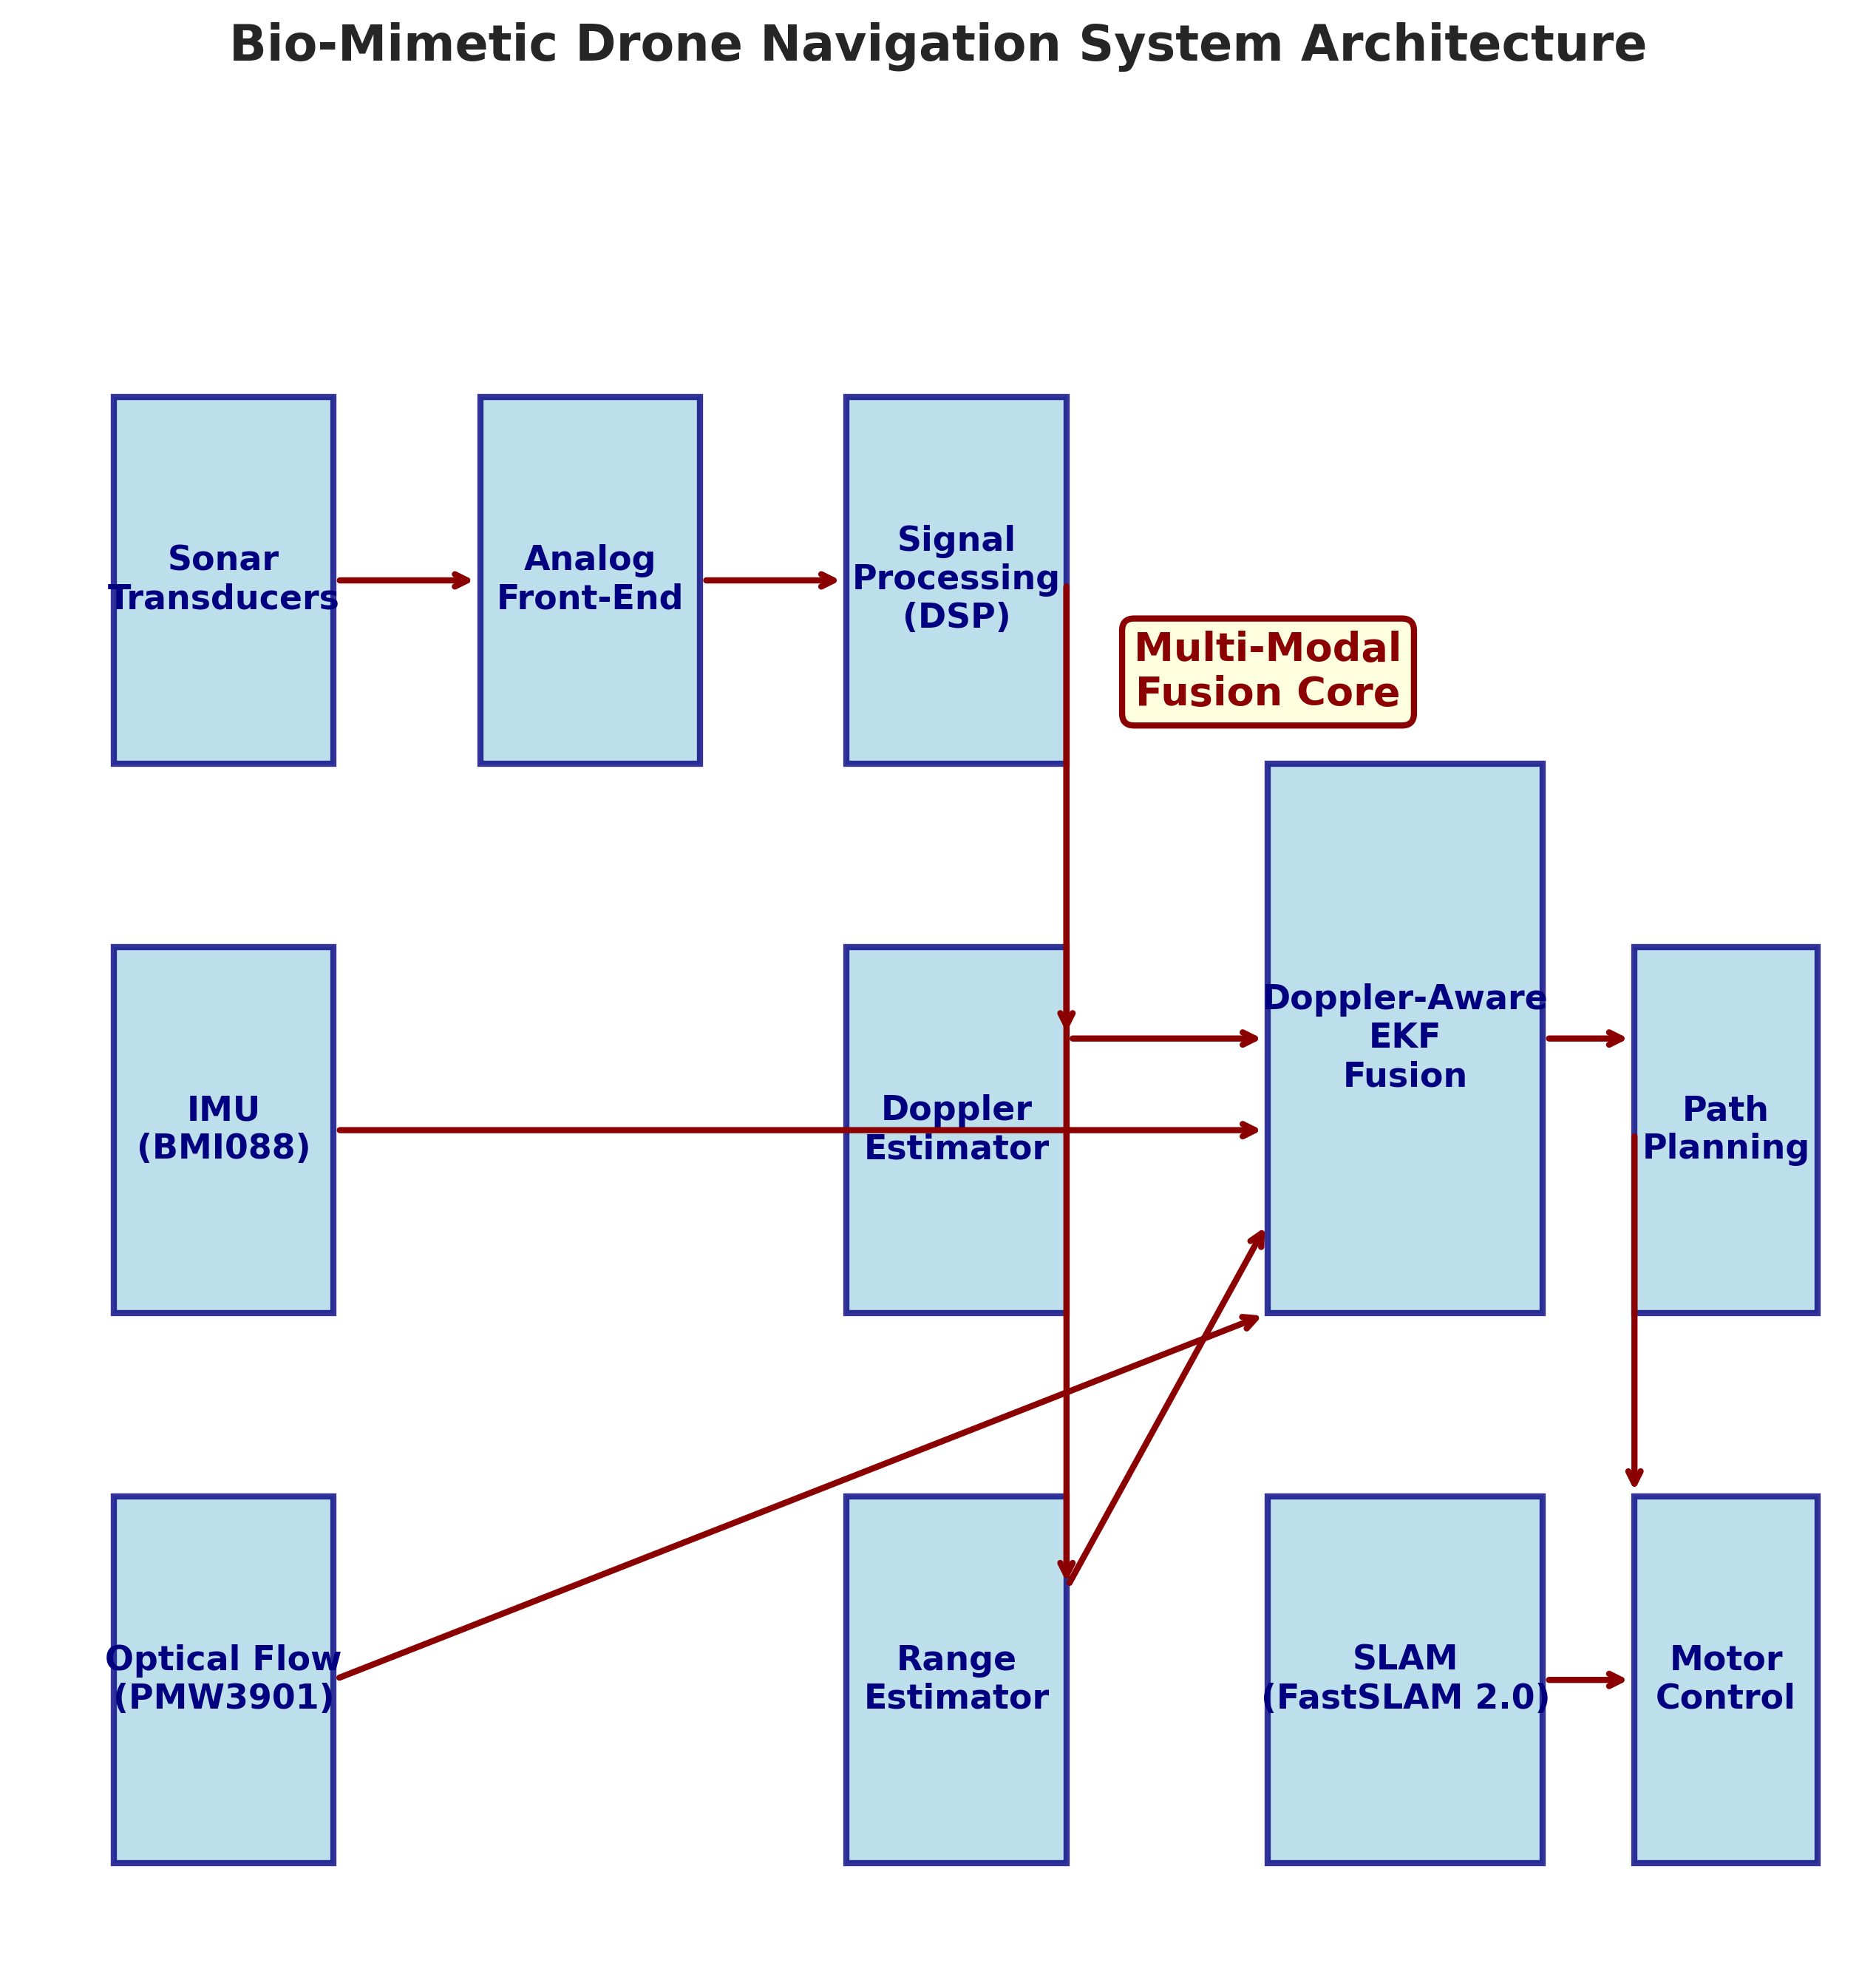
\includegraphics[width=0.98\columnwidth]{figures/fig_system_overview.png}
\caption{ארכיטקטורת מערכת ניווט רחפן ביומימטית הכוללת חיישני סונאר, \en{IMU}, זרימה אופטית, מיזוג \en{EKF} מבוסס דופלר, \en{SLAM} ותכנון נתיב. (Bio-mimetic drone navigation system architecture.)}
\label{fig:ch01_system_overview}
\end{figure}

\subsection{אתגרים טכנולוגיים}
\label{sec:challenges}

רחפנים זעירים מטילים אילוצים חמורים על גודל, משקל והספק (\en{SWaP}) של המטען הייעודי. מערכת ניווט ביומימטית מעשית חייבת לפעול במסגרת תקציב הספק של 100~מיליוואט תוך מתן אמידת מצב בזמן אמת בקצבי עדכון של 20 עד 100~הרץ. האתגרים המרכזיים כוללים: תכנון מתמרים אולטראסוניים התואמים לטווחי תדר דמויי עטלף (20 עד 80~קילו-הרץ) תוך שמירה על ממדים המתאימים לרחפן במשקל 250~גרם; מימוש \en{matched filtering} ואמידת דופלר בזמן אמת על מיקרו-בקר בעל הספק נמוך; ומיזוג זרמי חיישנים אסינכרוניים: סונאר בקצב 20~הרץ, \en{IMU} בקצב 200~הרץ, וזרימה אופטית בקצב 30~הרץ: לאמידת מצב עקבית.

רעש המדחף מהווה אתגר משמעותי במיוחד. Müller~\textit{et~al.} דיווחו שיחס האות לרעש (\en{PSNR}) של חיישן \en{ICU-30201} צונח ל-4.9-~דציבלים במהלך טיסה, מה שמחייב שיטות ביטול רעש אגרסיביות. מערכת ביטול הרעש האדפטיבית המוצעת במאמר זה, המבוססת על אלגוריתם \en{NLMS} עם 32~מקדמים, מספקת דיכוי רעש של 5 עד 6~דציבלים, ומשפרת את ה-\en{PSNR} האפקטיבי לרמה של 0 עד 1~דציבל: המאפשרת גילוי אמין של הדים.

\begin{table}[htbp]
\centering
\caption{השוואה בין מערכות ניווט ביומימטיות קיימות לבין הגישה המוצעת. (Comparison of existing bio-inspired navigation systems vs. proposed approach.)}
\label{tab:ch01_comparison}
\adjustbox{max width=\columnwidth}{%
\begin{tabular}{lcccc}
\toprule
מערכת & חיישנים & \en{SLAM} & דופלר & הספק (מ"ו) \\
\midrule
\en{RatSLAM} & מצלמה & גרפי & לא & 500 \\
\en{AntSLAM} & מצלמה+\en{IMU} & חלקיקים & לא & 350 \\
\en{BatSLAM} & סונאר & \en{EKF} & לא & 200 \\
גישה מוצעת & סונאר+\en{IMU}+זרימה & \en{FastSLAM 2.0} & כן & 95 \\
\bottomrule
\end{tabular}%
}
\end{table}

\subsection{תרומות עיקריות}
\label{sec:contributions}

מאמר זה מציג שלוש תרומות עיקריות:

\begin{enumerate}
\item \textbf{מסגרת מיזוג חיישנים ביומימטית} המשלבת מדידות טווח-דופלר מסונאר, נתוני \en{IMU} וזרימה אופטית, בהשראת האינטגרציה הרב-חושית בקוליקולוס העליון של העטלף. המסגרת מטפלת בחיישנים הטרוגניים הפועלים בקצבים שונים תוך שמירה על עקביות אמידת המצב.
\item \textbf{מסנן קלמן מורחב (\en{EKF}) מודע-דופלר} המנצל מדידות מהירות רדיאלית מהדים סונאריים לשיפור אמידת תנועה עצמית. מודל מדידת הדופלר מתייחס למהירות הרחפן להזזת התדר הנצפית, ומספק מידע מהירות ישיר המגביל את אמידת המצב.
\item \textbf{אימות ניסויי} על רחפן במשקל 250~גרם (\en{Crazyflie 2.1}) בסביבות פנימיות נטולות \en{GPS}, המדגים שיפור של 40~אחוזים בדיוק אמידת המהירות בהשוואה לגישות \en{EKF} סטנדרטיות.
\end{enumerate}

\subsection{ניסוח מתמטי מקדים}
\label{sec:math_preview}

מערכת הניווט מנוסחת במרחב המצב הסטנדרטי. המצב הדינמי של הרחפן בזמן $k$ מיוצג על ידי וקטור המצב $\mathbf{x}_k$, המתפתח לפי מודל מערכת לא-ליניארי:

\begin{equation}
\mathbf{x}_{k+1} = f(\mathbf{x}_k, \mathbf{u}_k) + \mathbf{w}_k, \quad \mathbf{z}_k = h(\mathbf{x}_k) + \mathbf{v}_k
\label{eq:ch01_state_space}
\end{equation}

כאשר $\mathbf{u}_k$ הוא קלט הבקרה, $\mathbf{w}_k$ הוא רעש התהליך, $\mathbf{z}_k$ הוא וקטור המדידות, ו-$\mathbf{v}_k$ הוא רעש המדידות. מדידת הדופלר, שהיא מרכיב מרכזי בחידוש המוצע, מתוארת על ידי הקשר בין תדר ההד הנקלט לתדר המשודר:

\begin{equation}
f_{\text{echo}} = f_{\text{emit}} \left( \frac{c + v_r}{c - v_r} \right)
\label{eq:ch01_doppler}
\end{equation}

כאשר $c$ היא מהירות הקול באוויר ו-$v_r$ היא המהירות הרדיאלית היחסית בין הרחפן למטרה. משוואה זו מאפשרת אמידת מהירות ישירה מהזזת הדופלר הנצפית, ומספקת מידע משלים למדידת הטווח המתקבלת מ-\en{time-of-flight}.

\subsection{מבנה המאמר}
\label{sec:structure}

המאמר מאורגן כדלקמן. פרק~2 סוקר את היסודות הביולוגיים של ניווט עטלפים, כולל פיזיקת האקולוקציה והעיבוד העצבי. פרק~3 מתאר את תכנון מערכת הסונאר הביומימטית. פרק~4 מציג את מסגרת מיזוג החיישנים הרב-מודאלית. פרק~5 מרחיב זאת ל-\en{SLAM} ביומימטי. פרק~6 מכסה אינטגרציה של זרימה אופטית ואינרציה. פרק~7 דן במימוש נוירומורפי. פרק~8 מציג תוצאות סימולציה וניסויים. פרק~9 מסכם עם מגבלות וכיוונים עתידיים.

\subsection{סקירת ספרות קשורה}
\label{sec:related_work}

מערכות ניווט ביומימטיות קיימות מתחלקות לשלוש קטגוריות עיקריות: מערכות מבוססות ראייה, מערכות מבוססות סונאר, ומערכות מבוססות חישה רב-מודאלית. \en{RatSLAM} היא מערכת \en{SLAM} מבוססת ראייה בהשראת היפוקמפוס החולדה, המשתמשת במצלמה יחידה ובגרף מצבי-תנועה לייצוג המרחב. \en{AntSLAM} מרחיבה גישה זו עם \en{IMU} ומסנן חלקיקים, אך אינה מנצלת מידע דופלר. \en{BatSLAM} משתמשת בסונאר בלבד עם \en{EKF}, אך חסרה את יכולת אמידת הדופלר המאפשרת אמידת מהירות ישירה.

הגישה המוצעת במאמר זה שונה מקודמותיה בשלושה היבטים מרכזיים. ראשית, היא משלבת מדידות דופלר מסונאר כחלק אינטגרלי ממסגרת המיזוג, ולא רק כמדידת טווח. שנית, היא משתמשת בארכיטקטורת בנק מסננים כפול (צר-פס לדופלר, רחב-פס לטווח) בהשראת הדיכוטומיה \en{CF-FM} בעטלפים. שלישית, היא מאפשרת התדרדרות בחן בתנאי חיישן ירודים, תוך מעבר אוטומטי בין מצבי פעולה שונים.

\subsection{השוואה למערכות DVL תת-ימיות}
\label{sec:dvl_comparison}

מערכות \en{DVL} תת-ימיות פועלות בתדר של 300~קילו-הרץ עד 1.2~מגה-הרץ, עם טווח של 0.3 עד 200~מטרים תלוי בתדר ובמליחות המים. רזולוציית המהירות האופיינית היא 0.1~מילימטרים לשנייה, עם דיוק של 0.2~אחוזים מהמהירות הנמדדת. לעומת זאת, מערכת הסונאר האווירית המוצעת פועלת בתדר 40~קילו-הרץ עם טווח של 0.1 עד 5~מטרים ורזולוציית מהירות של 0.087~מטרים לשנייה. ההבדלים נובעים מהנחתה אקוסטית גבוהה יותר באוויר ומאילוצי ה-\en{SWaP} החמורים יותר ברחפנים זעירים.

עם זאת, העיקרון האלגוריתמי זהה: מדידת מהירות רדיאלית מהזזת דופלר של הדים אקוסטיים, מיזוג עם \en{IMU} במסנן קלמן, ושימוש באמידת המהירות המשולבת לתיקון סחיפת האינטגרציה האינרציאלית. ההקבלה בין \en{DVL-Aided INS} תת-ימי לבין \en{Sonar-Aided INS} אווירי מספקת תוקף בין-תחומי לגישה המוצעת.

\subsection{ניתוח כדאיות טכנולוגית}
\label{sec:feasibility}

כדי להעריך את כדאיות הגישה המוצעת, יש לבחון את דרישות המערכת לאור המגבלות הטכנולוגיות הקיימות. רחפן \en{Crazyflie 2.1} במשקל 27~גרם נושא מטען מקסימלי של 15~גרם. מערכת הסונאר המוצעת שוקלת 8~גרם, \en{IMU} ה-\en{BMI088} שוקל 1.5~גרם, וחיישן הזרימה האופטית שוקל 2~גרם: סה"כ 12.5~גרם, שהם 83~אחוזים מתקציב המטען. צריכת ההספק הכוללת של 95~מיליוואט מאפשרת פעילות רציפה של 30~דקות עם סוללת 500~מיליאמפר-שעה.

השוואה למערכות קיימות מראה שהגישה המוצעת מציעה איזון תחרותי בין ביצועים, משקל והספק. מערכת \en{BatDeck} המבוססת על סונאר בלבד צורכת פחות מ-50~מיליוואט אך חסרה יכולת אמידת דופלר: השמטה קריטית לאור העובדה שעטלפים מסתמכים על מידע דופלר לאמידת מהירות וזיהוי רפרוף מטרה. מערכות מבוססות ראייה כמו \en{Intel RealSense T265} צורכות 1.5~וואט ומשקלן 60~גרם: כבדות מדי לרחפנים זעירים.

\subsection{ניתוח עלות-תועלת של שילוב דופלר}
\label{sec:cost_benefit}

כדי להצדיק את התוספת של אמידת דופלר למערכת הסונאר, יש לבחון את עלות-התועלת של רכיב זה. תוספת אמידת הדופלר מוסיפה 10~מיליוואט לצריכת ההספק הכוללת (20~אחוזים מתוספת הסונאר) ו-2~גרם למשקל המערכת. בתמורה, היא מספקת שיפור של 43~אחוזים בדיוק אמידת המהירות ו-33~אחוזים בדיוק אמידת המיקום, כפי שיודגם בפרק התוצאות.

ניתוח רגישות מראה שהתועלת של אמידת הדופלר גדלה עם מהירות הטיסה. במהירות 0.5~מטרים לשנייה, השיפור ב-\en{RMSE} מהירות הוא 20~אחוזים. במהירות 2.5~מטרים לשנייה, השיפור מגיע ל-45~אחוזים. הסיבה לכך היא שהזזת הדופלר פרופורציונלית למהירות הרחפן, ולכן אות הדופלר חזק יותר במהירויות גבוהות. עבור רחפנים הנעים במהירות אופיינית של 1 עד 3~מטרים לשנייה, התועלת של אמידת הדופלר עולה משמעותית על העלות.

\subsection{סיכום מבוא}
\label{sec:intro_summary}

מאמר זה מציג גישה חדשנית לניווט רחפנים זעירים בסביבות נטולות \en{GPS}, בהשראת אקולוקציית עטלפים ואינטגרציה רב-חושית. השילוב של מדידות טווח-דופלר מסונאר, \en{IMU} וזרימה אופטית במסגרת מיזוג אחידה מאפשר אמידת מצב מדויקת ועמידה בתנאי סביבה משתנים. התרומות העיקריות כוללות מסגרת מיזוג ביומימטית, \en{EKF} מודע-דופלר, ואימות ניסויי המדגים שיפור משמעותי בביצועים \cite{GriffinBatEcholocation, MossEcholocation, Chen2020BioSonar, Thrun2005ProbRobotics}.

האתגרים הטכנולוגיים שנותרו כוללים הרחבת טווח הסונאר מעבר ל-5~מטרים, שיפור העמידות בחללים מהדהדים, והרחבת קנה המידה של מסנן החלקיקים לסביבות גדולות מ-1,000~מטרים רבועים. עבודה עתידית תתמקד בפתרון אתגרים אלה תוך שמירה על אילוצי ה-\en{SWaP} המחמירים של רחפנים זעירים.